% Options for packages loaded elsewhere
\PassOptionsToPackage{unicode}{hyperref}
\PassOptionsToPackage{hyphens}{url}
%
\documentclass[
]{article}
\usepackage{amsmath,amssymb}
\usepackage{lmodern}
\usepackage{ifxetex,ifluatex}
\ifnum 0\ifxetex 1\fi\ifluatex 1\fi=0 % if pdftex
  \usepackage[T1]{fontenc}
  \usepackage[utf8]{inputenc}
  \usepackage{textcomp} % provide euro and other symbols
\else % if luatex or xetex
  \usepackage{unicode-math}
  \defaultfontfeatures{Scale=MatchLowercase}
  \defaultfontfeatures[\rmfamily]{Ligatures=TeX,Scale=1}
\fi
% Use upquote if available, for straight quotes in verbatim environments
\IfFileExists{upquote.sty}{\usepackage{upquote}}{}
\IfFileExists{microtype.sty}{% use microtype if available
  \usepackage[]{microtype}
  \UseMicrotypeSet[protrusion]{basicmath} % disable protrusion for tt fonts
}{}
\makeatletter
\@ifundefined{KOMAClassName}{% if non-KOMA class
  \IfFileExists{parskip.sty}{%
    \usepackage{parskip}
  }{% else
    \setlength{\parindent}{0pt}
    \setlength{\parskip}{6pt plus 2pt minus 1pt}}
}{% if KOMA class
  \KOMAoptions{parskip=half}}
\makeatother
\usepackage{xcolor}
\IfFileExists{xurl.sty}{\usepackage{xurl}}{} % add URL line breaks if available
\IfFileExists{bookmark.sty}{\usepackage{bookmark}}{\usepackage{hyperref}}
\hypersetup{
  pdftitle={Subsetting Data in R},
  hidelinks,
  pdfcreator={LaTeX via pandoc}}
\urlstyle{same} % disable monospaced font for URLs
\usepackage[margin=1in]{geometry}
\usepackage{color}
\usepackage{fancyvrb}
\newcommand{\VerbBar}{|}
\newcommand{\VERB}{\Verb[commandchars=\\\{\}]}
\DefineVerbatimEnvironment{Highlighting}{Verbatim}{commandchars=\\\{\}}
% Add ',fontsize=\small' for more characters per line
\usepackage{framed}
\definecolor{shadecolor}{RGB}{248,248,248}
\newenvironment{Shaded}{\begin{snugshade}}{\end{snugshade}}
\newcommand{\AlertTok}[1]{\textcolor[rgb]{0.94,0.16,0.16}{#1}}
\newcommand{\AnnotationTok}[1]{\textcolor[rgb]{0.56,0.35,0.01}{\textbf{\textit{#1}}}}
\newcommand{\AttributeTok}[1]{\textcolor[rgb]{0.77,0.63,0.00}{#1}}
\newcommand{\BaseNTok}[1]{\textcolor[rgb]{0.00,0.00,0.81}{#1}}
\newcommand{\BuiltInTok}[1]{#1}
\newcommand{\CharTok}[1]{\textcolor[rgb]{0.31,0.60,0.02}{#1}}
\newcommand{\CommentTok}[1]{\textcolor[rgb]{0.56,0.35,0.01}{\textit{#1}}}
\newcommand{\CommentVarTok}[1]{\textcolor[rgb]{0.56,0.35,0.01}{\textbf{\textit{#1}}}}
\newcommand{\ConstantTok}[1]{\textcolor[rgb]{0.00,0.00,0.00}{#1}}
\newcommand{\ControlFlowTok}[1]{\textcolor[rgb]{0.13,0.29,0.53}{\textbf{#1}}}
\newcommand{\DataTypeTok}[1]{\textcolor[rgb]{0.13,0.29,0.53}{#1}}
\newcommand{\DecValTok}[1]{\textcolor[rgb]{0.00,0.00,0.81}{#1}}
\newcommand{\DocumentationTok}[1]{\textcolor[rgb]{0.56,0.35,0.01}{\textbf{\textit{#1}}}}
\newcommand{\ErrorTok}[1]{\textcolor[rgb]{0.64,0.00,0.00}{\textbf{#1}}}
\newcommand{\ExtensionTok}[1]{#1}
\newcommand{\FloatTok}[1]{\textcolor[rgb]{0.00,0.00,0.81}{#1}}
\newcommand{\FunctionTok}[1]{\textcolor[rgb]{0.00,0.00,0.00}{#1}}
\newcommand{\ImportTok}[1]{#1}
\newcommand{\InformationTok}[1]{\textcolor[rgb]{0.56,0.35,0.01}{\textbf{\textit{#1}}}}
\newcommand{\KeywordTok}[1]{\textcolor[rgb]{0.13,0.29,0.53}{\textbf{#1}}}
\newcommand{\NormalTok}[1]{#1}
\newcommand{\OperatorTok}[1]{\textcolor[rgb]{0.81,0.36,0.00}{\textbf{#1}}}
\newcommand{\OtherTok}[1]{\textcolor[rgb]{0.56,0.35,0.01}{#1}}
\newcommand{\PreprocessorTok}[1]{\textcolor[rgb]{0.56,0.35,0.01}{\textit{#1}}}
\newcommand{\RegionMarkerTok}[1]{#1}
\newcommand{\SpecialCharTok}[1]{\textcolor[rgb]{0.00,0.00,0.00}{#1}}
\newcommand{\SpecialStringTok}[1]{\textcolor[rgb]{0.31,0.60,0.02}{#1}}
\newcommand{\StringTok}[1]{\textcolor[rgb]{0.31,0.60,0.02}{#1}}
\newcommand{\VariableTok}[1]{\textcolor[rgb]{0.00,0.00,0.00}{#1}}
\newcommand{\VerbatimStringTok}[1]{\textcolor[rgb]{0.31,0.60,0.02}{#1}}
\newcommand{\WarningTok}[1]{\textcolor[rgb]{0.56,0.35,0.01}{\textbf{\textit{#1}}}}
\usepackage{graphicx}
\makeatletter
\def\maxwidth{\ifdim\Gin@nat@width>\linewidth\linewidth\else\Gin@nat@width\fi}
\def\maxheight{\ifdim\Gin@nat@height>\textheight\textheight\else\Gin@nat@height\fi}
\makeatother
% Scale images if necessary, so that they will not overflow the page
% margins by default, and it is still possible to overwrite the defaults
% using explicit options in \includegraphics[width, height, ...]{}
\setkeys{Gin}{width=\maxwidth,height=\maxheight,keepaspectratio}
% Set default figure placement to htbp
\makeatletter
\def\fps@figure{htbp}
\makeatother
\setlength{\emergencystretch}{3em} % prevent overfull lines
\providecommand{\tightlist}{%
  \setlength{\itemsep}{0pt}\setlength{\parskip}{0pt}}
\setcounter{secnumdepth}{-\maxdimen} % remove section numbering
\ifluatex
  \usepackage{selnolig}  % disable illegal ligatures
\fi

\title{Subsetting Data in R}
\author{}
\date{\vspace{-2.5em}}

\begin{document}
\maketitle

\hypertarget{overview}{%
\subsection{Overview}\label{overview}}

In this module, we will show you how to:

\begin{enumerate}
\def\labelenumi{\arabic{enumi}.}
\tightlist
\item
  Look at your data in different ways
\item
  Create a data frame and a tibble
\item
  Create new variables/make rownames a column
\item
  Rename columns of a data frame
\item
  Subset rows of a data frame
\item
  Subset columns of a data frame
\item
  Add/remove new columns to a data frame
\item
  Order the columns of a data frame
\item
  Order the rows of a data frame
\end{enumerate}

\hypertarget{setup}{%
\subsection{Setup}\label{setup}}

We will largely focus on the \texttt{dplyr} package which is part of the
\texttt{tidyverse}.

\begin{center}\includegraphics[width=0.25\linewidth]{https://tidyverse.tidyverse.org/logo} \end{center}

Some resources on how to use \texttt{dplyr}:

\begin{itemize}
\tightlist
\item
  \url{https://dplyr.tidyverse.org/}
\item
  \url{https://cran.r-project.org/web/packages/dplyr/vignettes/dplyr.html}
\item
  \url{https://www.opencasestudies.org/}
\end{itemize}

\hypertarget{why-dplyr}{%
\subsection{Why dplyr?}\label{why-dplyr}}

\begin{center}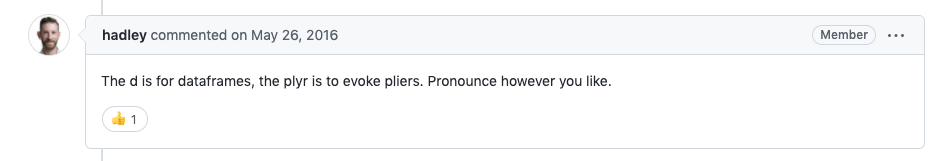
\includegraphics[width=1\linewidth]{images/dplyr} \end{center}

The \texttt{dplyr} package is one of the most helpful packages for
altering your data to get it into a form that is useful for creating
visualizations, summarizing, or more deeply analyzing.

So you can imagine using pliers on your data.

\hypertarget{loading-in-dplyr-and-tidyverse}{%
\subsection{Loading in dplyr and
tidyverse}\label{loading-in-dplyr-and-tidyverse}}

See this website for a list of the packages included in the
\texttt{tidyverse}: \url{https://www.tidyverse.org/packages/}

\begin{Shaded}
\begin{Highlighting}[]
\FunctionTok{library}\NormalTok{(tidyverse) }\CommentTok{\# loads dplyr and other packages!}
\end{Highlighting}
\end{Shaded}

\hypertarget{getting-data-to-work-with}{%
\subsection{Getting data to work with}\label{getting-data-to-work-with}}

Here we use one of the datasets that comes with base R called
\texttt{mtcars}. We will now create a toy data frame named \texttt{df}
using this data. This way we can alter \texttt{df} without worrying
about changing \texttt{mtcars}.

\begin{Shaded}
\begin{Highlighting}[]
\NormalTok{df }\OtherTok{\textless{}{-}}\NormalTok{ mtcars }\CommentTok{\# df is a copy of mtcars}
\FunctionTok{head}\NormalTok{(df) }\CommentTok{\# changing df does **not** change mtcars!}
\end{Highlighting}
\end{Shaded}

\begin{verbatim}
                   mpg cyl disp  hp drat    wt  qsec vs am gear carb
Mazda RX4         21.0   6  160 110 3.90 2.620 16.46  0  1    4    4
Mazda RX4 Wag     21.0   6  160 110 3.90 2.875 17.02  0  1    4    4
Datsun 710        22.8   4  108  93 3.85 2.320 18.61  1  1    4    1
Hornet 4 Drive    21.4   6  258 110 3.08 3.215 19.44  1  0    3    1
Hornet Sportabout 18.7   8  360 175 3.15 3.440 17.02  0  0    3    2
Valiant           18.1   6  225 105 2.76 3.460 20.22  1  0    3    1
\end{verbatim}

\hypertarget{checking-the-data-dim}{%
\subsection{\texorpdfstring{Checking the data
\texttt{dim()}}{Checking the data dim()}}\label{checking-the-data-dim}}

The \texttt{dim()} , \texttt{nrow()}, and \texttt{ncol()} functions are
good options to check the dimensions of your data before moving forward.

\begin{Shaded}
\begin{Highlighting}[]
\FunctionTok{dim}\NormalTok{(df) }\CommentTok{\# rows, columns}
\end{Highlighting}
\end{Shaded}

\begin{verbatim}
[1] 32 11
\end{verbatim}

\begin{Shaded}
\begin{Highlighting}[]
\FunctionTok{nrow}\NormalTok{(df) }\CommentTok{\# number of rows}
\end{Highlighting}
\end{Shaded}

\begin{verbatim}
[1] 32
\end{verbatim}

\begin{Shaded}
\begin{Highlighting}[]
\FunctionTok{ncol}\NormalTok{(df) }\CommentTok{\# number of columns}
\end{Highlighting}
\end{Shaded}

\begin{verbatim}
[1] 11
\end{verbatim}

\hypertarget{checking-the-data-glimpse}{%
\subsection{\texorpdfstring{Checking the data:
\texttt{glimpse()}}{Checking the data: glimpse()}}\label{checking-the-data-glimpse}}

In addition to \texttt{head()} and \texttt{tail()}, the
\texttt{glimpse()}function of the \texttt{dplyr} package is another
great function to look at your data.

\begin{Shaded}
\begin{Highlighting}[]
\FunctionTok{glimpse}\NormalTok{(df)}
\end{Highlighting}
\end{Shaded}

\begin{verbatim}
Rows: 32
Columns: 11
$ mpg  <dbl> 21.0, 21.0, 22.8, 21.4, 18.7, 18.1, 14.3, 24.4, 22.8, 19.2, 17.8,~
$ cyl  <dbl> 6, 6, 4, 6, 8, 6, 8, 4, 4, 6, 6, 8, 8, 8, 8, 8, 8, 4, 4, 4, 4, 8,~
$ disp <dbl> 160.0, 160.0, 108.0, 258.0, 360.0, 225.0, 360.0, 146.7, 140.8, 16~
$ hp   <dbl> 110, 110, 93, 110, 175, 105, 245, 62, 95, 123, 123, 180, 180, 180~
$ drat <dbl> 3.90, 3.90, 3.85, 3.08, 3.15, 2.76, 3.21, 3.69, 3.92, 3.92, 3.92,~
$ wt   <dbl> 2.620, 2.875, 2.320, 3.215, 3.440, 3.460, 3.570, 3.190, 3.150, 3.~
$ qsec <dbl> 16.46, 17.02, 18.61, 19.44, 17.02, 20.22, 15.84, 20.00, 22.90, 18~
$ vs   <dbl> 0, 0, 1, 1, 0, 1, 0, 1, 1, 1, 1, 0, 0, 0, 0, 0, 0, 1, 1, 1, 1, 0,~
$ am   <dbl> 1, 1, 1, 0, 0, 0, 0, 0, 0, 0, 0, 0, 0, 0, 0, 0, 0, 1, 1, 1, 0, 0,~
$ gear <dbl> 4, 4, 4, 3, 3, 3, 3, 4, 4, 4, 4, 3, 3, 3, 3, 3, 3, 4, 4, 4, 3, 3,~
$ carb <dbl> 4, 4, 1, 1, 2, 1, 4, 2, 2, 4, 4, 3, 3, 3, 4, 4, 4, 1, 2, 1, 1, 2,~
\end{verbatim}

\hypertarget{checking-your-data-slice_sample}{%
\subsection{\texorpdfstring{Checking your data:
\texttt{slice\_sample()}}{Checking your data: slice\_sample()}}\label{checking-your-data-slice_sample}}

What if you want to see the middle of your data? You can use the
\texttt{slice\_sample()} function of the \texttt{dplyr} package to see a
random set of rows. You can specify the number of rows with the
\texttt{n} argument or use a proportion with the \texttt{prop} argument.

\begin{Shaded}
\begin{Highlighting}[]
\FunctionTok{slice\_sample}\NormalTok{(df, }\AttributeTok{n =} \DecValTok{3}\NormalTok{)}
\end{Highlighting}
\end{Shaded}

\begin{verbatim}
             mpg cyl  disp  hp drat    wt  qsec vs am gear carb
Honda Civic 30.4   4  75.7  52 4.93 1.615 18.52  1  1    4    2
Camaro Z28  13.3   8 350.0 245 3.73 3.840 15.41  0  0    3    4
Duster 360  14.3   8 360.0 245 3.21 3.570 15.84  0  0    3    4
\end{verbatim}

\begin{Shaded}
\begin{Highlighting}[]
\FunctionTok{slice\_sample}\NormalTok{(df, }\AttributeTok{prop =}\NormalTok{ .}\DecValTok{2}\NormalTok{)}
\end{Highlighting}
\end{Shaded}

\begin{verbatim}
                mpg cyl  disp  hp drat    wt  qsec vs am gear carb
Maserati Bora  15.0   8 301.0 335 3.54 3.570 14.60  0  1    5    8
Mazda RX4      21.0   6 160.0 110 3.90 2.620 16.46  0  1    4    4
Lotus Europa   30.4   4  95.1 113 3.77 1.513 16.90  1  1    5    2
Valiant        18.1   6 225.0 105 2.76 3.460 20.22  1  0    3    1
Hornet 4 Drive 21.4   6 258.0 110 3.08 3.215 19.44  1  0    3    1
Datsun 710     22.8   4 108.0  93 3.85 2.320 18.61  1  1    4    1
\end{verbatim}

\hypertarget{making-data-framesbase-r-and-tibbles-tidyverse}{%
\section{Making data frames(base R) and tibbles
(tidyverse)}\label{making-data-framesbase-r-and-tibbles-tidyverse}}

\hypertarget{creating-data-frames-using-base-r-data-frame-function}{%
\subsection{Creating data frames using base R data frame
function}\label{creating-data-frames-using-base-r-data-frame-function}}

\begin{Shaded}
\begin{Highlighting}[]
\FunctionTok{data.frame}\NormalTok{(df)}
\end{Highlighting}
\end{Shaded}

\begin{verbatim}
                     mpg cyl  disp  hp drat    wt  qsec vs am gear carb
Mazda RX4           21.0   6 160.0 110 3.90 2.620 16.46  0  1    4    4
Mazda RX4 Wag       21.0   6 160.0 110 3.90 2.875 17.02  0  1    4    4
Datsun 710          22.8   4 108.0  93 3.85 2.320 18.61  1  1    4    1
Hornet 4 Drive      21.4   6 258.0 110 3.08 3.215 19.44  1  0    3    1
Hornet Sportabout   18.7   8 360.0 175 3.15 3.440 17.02  0  0    3    2
Valiant             18.1   6 225.0 105 2.76 3.460 20.22  1  0    3    1
Duster 360          14.3   8 360.0 245 3.21 3.570 15.84  0  0    3    4
Merc 240D           24.4   4 146.7  62 3.69 3.190 20.00  1  0    4    2
Merc 230            22.8   4 140.8  95 3.92 3.150 22.90  1  0    4    2
Merc 280            19.2   6 167.6 123 3.92 3.440 18.30  1  0    4    4
Merc 280C           17.8   6 167.6 123 3.92 3.440 18.90  1  0    4    4
Merc 450SE          16.4   8 275.8 180 3.07 4.070 17.40  0  0    3    3
Merc 450SL          17.3   8 275.8 180 3.07 3.730 17.60  0  0    3    3
Merc 450SLC         15.2   8 275.8 180 3.07 3.780 18.00  0  0    3    3
Cadillac Fleetwood  10.4   8 472.0 205 2.93 5.250 17.98  0  0    3    4
Lincoln Continental 10.4   8 460.0 215 3.00 5.424 17.82  0  0    3    4
Chrysler Imperial   14.7   8 440.0 230 3.23 5.345 17.42  0  0    3    4
Fiat 128            32.4   4  78.7  66 4.08 2.200 19.47  1  1    4    1
Honda Civic         30.4   4  75.7  52 4.93 1.615 18.52  1  1    4    2
Toyota Corolla      33.9   4  71.1  65 4.22 1.835 19.90  1  1    4    1
Toyota Corona       21.5   4 120.1  97 3.70 2.465 20.01  1  0    3    1
Dodge Challenger    15.5   8 318.0 150 2.76 3.520 16.87  0  0    3    2
AMC Javelin         15.2   8 304.0 150 3.15 3.435 17.30  0  0    3    2
Camaro Z28          13.3   8 350.0 245 3.73 3.840 15.41  0  0    3    4
Pontiac Firebird    19.2   8 400.0 175 3.08 3.845 17.05  0  0    3    2
Fiat X1-9           27.3   4  79.0  66 4.08 1.935 18.90  1  1    4    1
Porsche 914-2       26.0   4 120.3  91 4.43 2.140 16.70  0  1    5    2
Lotus Europa        30.4   4  95.1 113 3.77 1.513 16.90  1  1    5    2
Ford Pantera L      15.8   8 351.0 264 4.22 3.170 14.50  0  1    5    4
Ferrari Dino        19.7   6 145.0 175 3.62 2.770 15.50  0  1    5    6
Maserati Bora       15.0   8 301.0 335 3.54 3.570 14.60  0  1    5    8
Volvo 142E          21.4   4 121.0 109 4.11 2.780 18.60  1  1    4    2
\end{verbatim}

\hypertarget{keep-in-mind}{%
\subsection{Keep in mind\ldots{}}\label{keep-in-mind}}

Need to assign the output of the function to keep the result!

\begin{Shaded}
\begin{Highlighting}[]
\NormalTok{df\_updated }\OtherTok{\textless{}{-}}\FunctionTok{data.frame}\NormalTok{(df)}
\CommentTok{\# this would overwrite the existing df object}
\NormalTok{df}\OtherTok{\textless{}{-}}\FunctionTok{data.frame}\NormalTok{(df) }
\end{Highlighting}
\end{Shaded}

\hypertarget{or-create-a-data-frame-when-reading-in-the-file}{%
\subsection{Or create a data frame when reading in the
file}\label{or-create-a-data-frame-when-reading-in-the-file}}

Or directly when reading in a csv with the \texttt{read.csv()} function
(also base R)

\begin{Shaded}
\begin{Highlighting}[]
\CommentTok{\# function comes from base R {-} no package loading required}
\NormalTok{df\_example\_readr }\OtherTok{\textless{}{-}} \FunctionTok{read.csv}\NormalTok{(}\StringTok{"documents/data\_analysis/data\_file.csv"}\NormalTok{)}
\end{Highlighting}
\end{Shaded}

\hypertarget{tibble}{%
\subsection{tibble}\label{tibble}}

We can create a \textbf{fancier} version of the previous data frame
which can be really helpful.

\hypertarget{creating-a-tibble}{%
\subsection{\texorpdfstring{Creating a
\texttt{tibble}}{Creating a tibble}}\label{creating-a-tibble}}

If we would like to create a \texttt{tibble} (``fancy'' data frame), we
can using the \texttt{tibble()} function.

\begin{Shaded}
\begin{Highlighting}[]
\NormalTok{tbl }\OtherTok{\textless{}{-}}\NormalTok{ dplyr}\SpecialCharTok{::}\FunctionTok{tibble}\NormalTok{(df) }
\NormalTok{tbl}
\end{Highlighting}
\end{Shaded}

\begin{verbatim}
# A tibble: 32 x 11
     mpg   cyl  disp    hp  drat    wt  qsec    vs    am  gear  carb
   <dbl> <dbl> <dbl> <dbl> <dbl> <dbl> <dbl> <dbl> <dbl> <dbl> <dbl>
 1  21       6  160    110  3.9   2.62  16.5     0     1     4     4
 2  21       6  160    110  3.9   2.88  17.0     0     1     4     4
 3  22.8     4  108     93  3.85  2.32  18.6     1     1     4     1
 4  21.4     6  258    110  3.08  3.22  19.4     1     0     3     1
 5  18.7     8  360    175  3.15  3.44  17.0     0     0     3     2
 6  18.1     6  225    105  2.76  3.46  20.2     1     0     3     1
 7  14.3     8  360    245  3.21  3.57  15.8     0     0     3     4
 8  24.4     4  147.    62  3.69  3.19  20       1     0     4     2
 9  22.8     4  141.    95  3.92  3.15  22.9     1     0     4     2
10  19.2     6  168.   123  3.92  3.44  18.3     1     0     4     4
# ... with 22 more rows
\end{verbatim}

Note don't necessarily need to use \texttt{head()}- tibbles conveniently
print a portion of the data.

\hypertarget{tibbles-form-read_csv}{%
\subsection{tibbles form read\_csv()}\label{tibbles-form-read_csv}}

Alternatively we can read data files using the tidyverse with the
\texttt{read\_csv()} function of the \texttt{readr} package from the
\texttt{tidyverse} to make a tibble.

\begin{Shaded}
\begin{Highlighting}[]
\NormalTok{df\_example\_readr }\OtherTok{\textless{}{-}} \FunctionTok{read\_csv}\NormalTok{(}\StringTok{"documents/data\_analysis/data\_file.csv"}\NormalTok{)}
\end{Highlighting}
\end{Shaded}

You may start to notice how the tidyverse package work well together!

\hypertarget{summary-of-tibbles-and-data-frames}{%
\subsection{Summary of tibbles and data
frames}\label{summary-of-tibbles-and-data-frames}}

\textbf{Base R:}\\
Using \texttt{read.csv()} and \texttt{data.frame()} you can make data
frames

\textbf{Tidyverse (fancier version):}\\
Using \texttt{read\_csv()} and \texttt{tibble()} you can make tibbles

We generally recommend using tibbles, but you can do a lot with tibbles
too.

\hypertarget{data-frames-vs-tibbles}{%
\subsection{Data frames vs tibbles}\label{data-frames-vs-tibbles}}

In the ``tidy'' data format, rownames are removed. For example,
\texttt{df} has each car name as a row name. Here we use the
\texttt{head()} function to see the first 2 rows of each. In this case
we would want to make the rownames a new column first before making into
a tibble.

\begin{Shaded}
\begin{Highlighting}[]
\FunctionTok{head}\NormalTok{(df, }\DecValTok{2}\NormalTok{)}
\end{Highlighting}
\end{Shaded}

\begin{verbatim}
              mpg cyl disp  hp drat    wt  qsec vs am gear carb
Mazda RX4      21   6  160 110  3.9 2.620 16.46  0  1    4    4
Mazda RX4 Wag  21   6  160 110  3.9 2.875 17.02  0  1    4    4
\end{verbatim}

\begin{Shaded}
\begin{Highlighting}[]
\FunctionTok{head}\NormalTok{(}\FunctionTok{tibble}\NormalTok{(df), }\DecValTok{2}\NormalTok{)}
\end{Highlighting}
\end{Shaded}

\begin{verbatim}
# A tibble: 2 x 11
    mpg   cyl  disp    hp  drat    wt  qsec    vs    am  gear  carb
  <dbl> <dbl> <dbl> <dbl> <dbl> <dbl> <dbl> <dbl> <dbl> <dbl> <dbl>
1    21     6   160   110   3.9  2.62  16.5     0     1     4     4
2    21     6   160   110   3.9  2.88  17.0     0     1     4     4
\end{verbatim}

\hypertarget{rownames_to_column-function}{%
\subsection{rownames\_to\_column
function}\label{rownames_to_column-function}}

If you run into losing a variable contained in your row names, you can
also use \texttt{rownames\_to\_column} to add it before turning it into
a \texttt{tibble} to keep them:

\begin{Shaded}
\begin{Highlighting}[]
\FunctionTok{head}\NormalTok{(}\FunctionTok{rownames\_to\_column}\NormalTok{(df, }\AttributeTok{var =} \StringTok{"car"}\NormalTok{),  }\DecValTok{2}\NormalTok{)}
\end{Highlighting}
\end{Shaded}

\begin{verbatim}
            car mpg cyl disp  hp drat    wt  qsec vs am gear carb
1     Mazda RX4  21   6  160 110  3.9 2.620 16.46  0  1    4    4
2 Mazda RX4 Wag  21   6  160 110  3.9 2.875 17.02  0  1    4    4
\end{verbatim}

\begin{Shaded}
\begin{Highlighting}[]
\FunctionTok{head}\NormalTok{(}\FunctionTok{tibble}\NormalTok{(}\FunctionTok{rownames\_to\_column}\NormalTok{(df, }\AttributeTok{var =} \StringTok{"car"}\NormalTok{)),  }\DecValTok{2}\NormalTok{)}
\end{Highlighting}
\end{Shaded}

\begin{verbatim}
# A tibble: 2 x 12
  car            mpg   cyl  disp    hp  drat    wt  qsec    vs    am  gear  carb
  <chr>        <dbl> <dbl> <dbl> <dbl> <dbl> <dbl> <dbl> <dbl> <dbl> <dbl> <dbl>
1 Mazda RX4       21     6   160   110   3.9  2.62  16.5     0     1     4     4
2 Mazda RX4 W~    21     6   160   110   3.9  2.88  17.0     0     1     4     4
\end{verbatim}

\hypertarget{renaming-columns}{%
\section{Renaming Columns}\label{renaming-columns}}

\hypertarget{renaming-columns-of-a-data-frame-or-tibble}{%
\subsection{Renaming Columns of a data frame or
tibble}\label{renaming-columns-of-a-data-frame-or-tibble}}

To rename columns in \texttt{dplyr}, you can use the \texttt{rename}
function.

For example, let's rename mpg to MPG. Notice the new name is listed
\textbf{first}!

\begin{Shaded}
\begin{Highlighting}[]
\CommentTok{\# general format! not code!}
\NormalTok{\{data you are creating or changing\} }\OtherTok{\textless{}{-}} \FunctionTok{rename}\NormalTok{(\{data you are using\}, }
\NormalTok{                                        \{New Name\} }\OtherTok{=}\NormalTok{ \{Old name\})}
\end{Highlighting}
\end{Shaded}

\begin{Shaded}
\begin{Highlighting}[]
\NormalTok{df }\OtherTok{\textless{}{-}}\NormalTok{ dplyr}\SpecialCharTok{::}\FunctionTok{rename}\NormalTok{(df, }\AttributeTok{MPG =}\NormalTok{ mpg)}
\FunctionTok{head}\NormalTok{(df)}
\end{Highlighting}
\end{Shaded}

\begin{verbatim}
                   MPG cyl disp  hp drat    wt  qsec vs am gear carb
Mazda RX4         21.0   6  160 110 3.90 2.620 16.46  0  1    4    4
Mazda RX4 Wag     21.0   6  160 110 3.90 2.875 17.02  0  1    4    4
Datsun 710        22.8   4  108  93 3.85 2.320 18.61  1  1    4    1
Hornet 4 Drive    21.4   6  258 110 3.08 3.215 19.44  1  0    3    1
Hornet Sportabout 18.7   8  360 175 3.15 3.440 17.02  0  0    3    2
Valiant           18.1   6  225 105 2.76 3.460 20.22  1  0    3    1
\end{verbatim}

\hypertarget{renaming-all-columns-of-a-data-frame-dplyr}{%
\subsection{Renaming All Columns of a data frame:
dplyr}\label{renaming-all-columns-of-a-data-frame-dplyr}}

To rename all columns you use the \texttt{rename\_all()}. In this case
we will use \texttt{toupper()} to make all letters upper case. Could
also use \texttt{tolower()} function.

\begin{Shaded}
\begin{Highlighting}[]
\NormalTok{df\_upper }\OtherTok{\textless{}{-}}\NormalTok{ dplyr}\SpecialCharTok{::}\FunctionTok{rename\_all}\NormalTok{(df, toupper)}
\FunctionTok{head}\NormalTok{(df\_upper, }\DecValTok{3}\NormalTok{)}
\end{Highlighting}
\end{Shaded}

\begin{verbatim}
               MPG CYL DISP  HP DRAT    WT  QSEC VS AM GEAR CARB
Mazda RX4     21.0   6  160 110 3.90 2.620 16.46  0  1    4    4
Mazda RX4 Wag 21.0   6  160 110 3.90 2.875 17.02  0  1    4    4
Datsun 710    22.8   4  108  93 3.85 2.320 18.61  1  1    4    1
\end{verbatim}

\begin{Shaded}
\begin{Highlighting}[]
\NormalTok{df }\OtherTok{\textless{}{-}}\NormalTok{ dplyr}\SpecialCharTok{::}\FunctionTok{rename\_all}\NormalTok{(df, tolower)}
\FunctionTok{head}\NormalTok{(df, }\DecValTok{3}\NormalTok{)}
\end{Highlighting}
\end{Shaded}

\begin{verbatim}
               mpg cyl disp  hp drat    wt  qsec vs am gear carb
Mazda RX4     21.0   6  160 110 3.90 2.620 16.46  0  1    4    4
Mazda RX4 Wag 21.0   6  160 110 3.90 2.875 17.02  0  1    4    4
Datsun 710    22.8   4  108  93 3.85 2.320 18.61  1  1    4    1
\end{verbatim}

\hypertarget{lab-part-1}{%
\subsection{Lab Part 1}\label{lab-part-1}}

\href{http://https://jhudatascience.org/intro_to_R_class/index.html}{Website}

\hypertarget{subsetting-columns}{%
\section{Subsetting Columns}\label{subsetting-columns}}

\hypertarget{subset-columns-of-a-data-frame}{%
\subsection{Subset columns of a data
frame:}\label{subset-columns-of-a-data-frame}}

We can grab the \texttt{carb} column using the \texttt{\$} operator.
This is the base R way to do this:

\begin{Shaded}
\begin{Highlighting}[]
\NormalTok{df}\SpecialCharTok{$}\NormalTok{carb}
\end{Highlighting}
\end{Shaded}

\begin{verbatim}
 [1] 4 4 1 1 2 1 4 2 2 4 4 3 3 3 4 4 4 1 2 1 1 2 2 4 2 1 2 2 4 6 8 2
\end{verbatim}

\hypertarget{subset-columns-of-a-data-frame---tidyverse-way}{%
\subsection{\texorpdfstring{Subset columns of a data frame -
\texttt{tidyverse}
way:}{Subset columns of a data frame - tidyverse way:}}\label{subset-columns-of-a-data-frame---tidyverse-way}}

To grab the \texttt{carb} column the \texttt{tidyverse} way we can use
the \texttt{pull} function:

\begin{Shaded}
\begin{Highlighting}[]
\FunctionTok{pull}\NormalTok{(df, carb)}
\end{Highlighting}
\end{Shaded}

\begin{verbatim}
 [1] 4 4 1 1 2 1 4 2 2 4 4 3 3 3 4 4 4 1 2 1 1 2 2 4 2 1 2 2 4 6 8 2
\end{verbatim}

\hypertarget{subset-columns-of-a-data-frame-dplyr}{%
\subsection{Subset columns of a data frame:
dplyr}\label{subset-columns-of-a-data-frame-dplyr}}

The \texttt{select} command from \texttt{dplyr} allows you to subset
(gives a \texttt{tibble}!)

\begin{Shaded}
\begin{Highlighting}[]
\FunctionTok{select}\NormalTok{(df, mpg)}
\end{Highlighting}
\end{Shaded}

\begin{verbatim}
                     mpg
Mazda RX4           21.0
Mazda RX4 Wag       21.0
Datsun 710          22.8
Hornet 4 Drive      21.4
Hornet Sportabout   18.7
Valiant             18.1
Duster 360          14.3
Merc 240D           24.4
Merc 230            22.8
Merc 280            19.2
Merc 280C           17.8
Merc 450SE          16.4
Merc 450SL          17.3
Merc 450SLC         15.2
Cadillac Fleetwood  10.4
Lincoln Continental 10.4
Chrysler Imperial   14.7
Fiat 128            32.4
Honda Civic         30.4
Toyota Corolla      33.9
Toyota Corona       21.5
Dodge Challenger    15.5
AMC Javelin         15.2
Camaro Z28          13.3
Pontiac Firebird    19.2
Fiat X1-9           27.3
Porsche 914-2       26.0
Lotus Europa        30.4
Ford Pantera L      15.8
Ferrari Dino        19.7
Maserati Bora       15.0
Volvo 142E          21.4
\end{verbatim}

\hypertarget{subset-columns-of-a-data-frame-dplyr-1}{%
\subsection{Subset columns of a data frame:
dplyr}\label{subset-columns-of-a-data-frame-dplyr-1}}

Note that if you want a single vector (not a \texttt{tibble}), use
\texttt{pull} or \texttt{\$}:

\begin{Shaded}
\begin{Highlighting}[]
\FunctionTok{pull}\NormalTok{(df, mpg)}
\end{Highlighting}
\end{Shaded}

\begin{verbatim}
 [1] 21.0 21.0 22.8 21.4 18.7 18.1 14.3 24.4 22.8 19.2 17.8 16.4 17.3 15.2 10.4
[16] 10.4 14.7 32.4 30.4 33.9 21.5 15.5 15.2 13.3 19.2 27.3 26.0 30.4 15.8 19.7
[31] 15.0 21.4
\end{verbatim}

\begin{Shaded}
\begin{Highlighting}[]
\CommentTok{\# pull with select works too!}

\FunctionTok{pull}\NormalTok{(}\FunctionTok{select}\NormalTok{(df,mpg))}
\end{Highlighting}
\end{Shaded}

\begin{verbatim}
 [1] 21.0 21.0 22.8 21.4 18.7 18.1 14.3 24.4 22.8 19.2 17.8 16.4 17.3 15.2 10.4
[16] 10.4 14.7 32.4 30.4 33.9 21.5 15.5 15.2 13.3 19.2 27.3 26.0 30.4 15.8 19.7
[31] 15.0 21.4
\end{verbatim}

\hypertarget{select-columns-of-a-data-frame-dplyr}{%
\subsection{Select columns of a data frame:
dplyr}\label{select-columns-of-a-data-frame-dplyr}}

The \texttt{select} command from \texttt{dplyr} allows you to subset
columns matching strings:

\begin{Shaded}
\begin{Highlighting}[]
\FunctionTok{select}\NormalTok{(df, mpg, cyl)}
\end{Highlighting}
\end{Shaded}

\begin{verbatim}
                     mpg cyl
Mazda RX4           21.0   6
Mazda RX4 Wag       21.0   6
Datsun 710          22.8   4
Hornet 4 Drive      21.4   6
Hornet Sportabout   18.7   8
Valiant             18.1   6
Duster 360          14.3   8
Merc 240D           24.4   4
Merc 230            22.8   4
Merc 280            19.2   6
Merc 280C           17.8   6
Merc 450SE          16.4   8
Merc 450SL          17.3   8
Merc 450SLC         15.2   8
Cadillac Fleetwood  10.4   8
Lincoln Continental 10.4   8
Chrysler Imperial   14.7   8
Fiat 128            32.4   4
Honda Civic         30.4   4
Toyota Corolla      33.9   4
Toyota Corona       21.5   4
Dodge Challenger    15.5   8
AMC Javelin         15.2   8
Camaro Z28          13.3   8
Pontiac Firebird    19.2   8
Fiat X1-9           27.3   4
Porsche 914-2       26.0   4
Lotus Europa        30.4   4
Ford Pantera L      15.8   8
Ferrari Dino        19.7   6
Maserati Bora       15.0   8
Volvo 142E          21.4   4
\end{verbatim}

\begin{Shaded}
\begin{Highlighting}[]
\FunctionTok{select}\NormalTok{(df, }\FunctionTok{starts\_with}\NormalTok{(}\StringTok{"c"}\NormalTok{))}
\end{Highlighting}
\end{Shaded}

\begin{verbatim}
                    cyl carb
Mazda RX4             6    4
Mazda RX4 Wag         6    4
Datsun 710            4    1
Hornet 4 Drive        6    1
Hornet Sportabout     8    2
Valiant               6    1
Duster 360            8    4
Merc 240D             4    2
Merc 230              4    2
Merc 280              6    4
Merc 280C             6    4
Merc 450SE            8    3
Merc 450SL            8    3
Merc 450SLC           8    3
Cadillac Fleetwood    8    4
Lincoln Continental   8    4
Chrysler Imperial     8    4
Fiat 128              4    1
Honda Civic           4    2
Toyota Corolla        4    1
Toyota Corona         4    1
Dodge Challenger      8    2
AMC Javelin           8    2
Camaro Z28            8    4
Pontiac Firebird      8    2
Fiat X1-9             4    1
Porsche 914-2         4    2
Lotus Europa          4    2
Ford Pantera L        8    4
Ferrari Dino          6    6
Maserati Bora         8    8
Volvo 142E            4    2
\end{verbatim}

\hypertarget{see-the-select-helpers}{%
\subsection{See the Select ``helpers''}\label{see-the-select-helpers}}

Here are a few:

\begin{Shaded}
\begin{Highlighting}[]
\FunctionTok{one\_of}\NormalTok{() }\CommentTok{\# if they exist}
\FunctionTok{last\_col}\NormalTok{()}
\FunctionTok{ends\_with}\NormalTok{()}
\FunctionTok{contains}\NormalTok{() }\CommentTok{\# like searching}
\end{Highlighting}
\end{Shaded}

Type \texttt{tidyselect::} in the console and see what RStudio suggests:

\begin{Shaded}
\begin{Highlighting}[]
\NormalTok{tidyslect}\SpecialCharTok{::} 
\end{Highlighting}
\end{Shaded}

\hypertarget{lab-part-2}{%
\subsection{Lab Part 2}\label{lab-part-2}}

\href{http://https://jhudatascience.org/intro_to_R_class/index.html}{Website}

\hypertarget{subsetting-rows}{%
\section{Subsetting Rows}\label{subsetting-rows}}

\hypertarget{subset-rows-of-a-data-frame-dplyr}{%
\subsection{Subset rows of a data frame:
dplyr}\label{subset-rows-of-a-data-frame-dplyr}}

The command in \texttt{dplyr} for subsetting rows is \texttt{filter}.

\begin{Shaded}
\begin{Highlighting}[]
\FunctionTok{filter}\NormalTok{(df, mpg }\SpecialCharTok{\textgreater{}} \DecValTok{20}\NormalTok{)}
\end{Highlighting}
\end{Shaded}

\begin{verbatim}
                mpg cyl  disp  hp drat    wt  qsec vs am gear carb
Mazda RX4      21.0   6 160.0 110 3.90 2.620 16.46  0  1    4    4
Mazda RX4 Wag  21.0   6 160.0 110 3.90 2.875 17.02  0  1    4    4
Datsun 710     22.8   4 108.0  93 3.85 2.320 18.61  1  1    4    1
Hornet 4 Drive 21.4   6 258.0 110 3.08 3.215 19.44  1  0    3    1
Merc 240D      24.4   4 146.7  62 3.69 3.190 20.00  1  0    4    2
Merc 230       22.8   4 140.8  95 3.92 3.150 22.90  1  0    4    2
Fiat 128       32.4   4  78.7  66 4.08 2.200 19.47  1  1    4    1
Honda Civic    30.4   4  75.7  52 4.93 1.615 18.52  1  1    4    2
Toyota Corolla 33.9   4  71.1  65 4.22 1.835 19.90  1  1    4    1
Toyota Corona  21.5   4 120.1  97 3.70 2.465 20.01  1  0    3    1
Fiat X1-9      27.3   4  79.0  66 4.08 1.935 18.90  1  1    4    1
Porsche 914-2  26.0   4 120.3  91 4.43 2.140 16.70  0  1    5    2
Lotus Europa   30.4   4  95.1 113 3.77 1.513 16.90  1  1    5    2
Volvo 142E     21.4   4 121.0 109 4.11 2.780 18.60  1  1    4    2
\end{verbatim}

Note, no \texttt{\$} or subsetting is necessary. R ``knows''
\texttt{mpg} refers to a column of \texttt{df}.

\hypertarget{subset-rows-of-a-data-frame-dplyr-1}{%
\subsection{Subset rows of a data frame:
dplyr}\label{subset-rows-of-a-data-frame-dplyr-1}}

You can have multiple logical conditions using the following:

\begin{itemize}
\tightlist
\item
  \texttt{==} : equals to
\item
  \texttt{!=}: not equal to (\texttt{!} : not/negation)
\item
  \texttt{\textgreater{}} / \texttt{\textless{}}: greater than / less
  than
\item
  \texttt{\textgreater{}=} or \texttt{\textless{}=}: greater than or
  equal to / less than or equal to
\item
  \texttt{\&} : AND
\item
  \texttt{\textbar{}} : OR
\end{itemize}

\hypertarget{subset-rows-of-a-data-frame-dplyr-2}{%
\subsection{Subset rows of a data frame:
dplyr}\label{subset-rows-of-a-data-frame-dplyr-2}}

The \texttt{\%in\%} operator can be used find values from a pre-made
list (using \texttt{c()}):

\begin{Shaded}
\begin{Highlighting}[]
\FunctionTok{filter}\NormalTok{(df, mpg }\SpecialCharTok{\%in\%} \FunctionTok{c}\NormalTok{(}\DecValTok{20}\NormalTok{,}\DecValTok{21}\NormalTok{,}\DecValTok{22}\NormalTok{))}
\end{Highlighting}
\end{Shaded}

\begin{verbatim}
              mpg cyl disp  hp drat    wt  qsec vs am gear carb
Mazda RX4      21   6  160 110  3.9 2.620 16.46  0  1    4    4
Mazda RX4 Wag  21   6  160 110  3.9 2.875 17.02  0  1    4    4
\end{verbatim}

\hypertarget{subset-rows-of-a-data-frame-dplyr-3}{%
\subsection{Subset rows of a data frame:
dplyr}\label{subset-rows-of-a-data-frame-dplyr-3}}

You can filter by two conditions using \texttt{\&} or commas:

\begin{Shaded}
\begin{Highlighting}[]
\FunctionTok{filter}\NormalTok{(df, mpg }\SpecialCharTok{\textgreater{}} \DecValTok{20} \SpecialCharTok{\&}\NormalTok{ cyl }\SpecialCharTok{==} \DecValTok{4}\NormalTok{)}
\end{Highlighting}
\end{Shaded}

\begin{verbatim}
                mpg cyl  disp  hp drat    wt  qsec vs am gear carb
Datsun 710     22.8   4 108.0  93 3.85 2.320 18.61  1  1    4    1
Merc 240D      24.4   4 146.7  62 3.69 3.190 20.00  1  0    4    2
Merc 230       22.8   4 140.8  95 3.92 3.150 22.90  1  0    4    2
Fiat 128       32.4   4  78.7  66 4.08 2.200 19.47  1  1    4    1
Honda Civic    30.4   4  75.7  52 4.93 1.615 18.52  1  1    4    2
Toyota Corolla 33.9   4  71.1  65 4.22 1.835 19.90  1  1    4    1
Toyota Corona  21.5   4 120.1  97 3.70 2.465 20.01  1  0    3    1
Fiat X1-9      27.3   4  79.0  66 4.08 1.935 18.90  1  1    4    1
Porsche 914-2  26.0   4 120.3  91 4.43 2.140 16.70  0  1    5    2
Lotus Europa   30.4   4  95.1 113 3.77 1.513 16.90  1  1    5    2
Volvo 142E     21.4   4 121.0 109 4.11 2.780 18.60  1  1    4    2
\end{verbatim}

\begin{Shaded}
\begin{Highlighting}[]
\FunctionTok{filter}\NormalTok{(df, mpg }\SpecialCharTok{\textgreater{}} \DecValTok{20}\NormalTok{, cyl }\SpecialCharTok{==} \DecValTok{4}\NormalTok{)}
\end{Highlighting}
\end{Shaded}

\begin{verbatim}
                mpg cyl  disp  hp drat    wt  qsec vs am gear carb
Datsun 710     22.8   4 108.0  93 3.85 2.320 18.61  1  1    4    1
Merc 240D      24.4   4 146.7  62 3.69 3.190 20.00  1  0    4    2
Merc 230       22.8   4 140.8  95 3.92 3.150 22.90  1  0    4    2
Fiat 128       32.4   4  78.7  66 4.08 2.200 19.47  1  1    4    1
Honda Civic    30.4   4  75.7  52 4.93 1.615 18.52  1  1    4    2
Toyota Corolla 33.9   4  71.1  65 4.22 1.835 19.90  1  1    4    1
Toyota Corona  21.5   4 120.1  97 3.70 2.465 20.01  1  0    3    1
Fiat X1-9      27.3   4  79.0  66 4.08 1.935 18.90  1  1    4    1
Porsche 914-2  26.0   4 120.3  91 4.43 2.140 16.70  0  1    5    2
Lotus Europa   30.4   4  95.1 113 3.77 1.513 16.90  1  1    5    2
Volvo 142E     21.4   4 121.0 109 4.11 2.780 18.60  1  1    4    2
\end{verbatim}

\hypertarget{subset-rows-of-a-data-frame-dplyr-4}{%
\subsection{Subset rows of a data frame:
dplyr}\label{subset-rows-of-a-data-frame-dplyr-4}}

If you want OR statements (meaning the data can meet either condition
does not need to meet both), you need to use the pipe
\texttt{\textbar{}} between conditions:

\begin{Shaded}
\begin{Highlighting}[]
\FunctionTok{filter}\NormalTok{(df, mpg }\SpecialCharTok{\textgreater{}} \DecValTok{20} \SpecialCharTok{|}\NormalTok{ cyl }\SpecialCharTok{==} \DecValTok{4}\NormalTok{)}
\end{Highlighting}
\end{Shaded}

\begin{verbatim}
                mpg cyl  disp  hp drat    wt  qsec vs am gear carb
Mazda RX4      21.0   6 160.0 110 3.90 2.620 16.46  0  1    4    4
Mazda RX4 Wag  21.0   6 160.0 110 3.90 2.875 17.02  0  1    4    4
Datsun 710     22.8   4 108.0  93 3.85 2.320 18.61  1  1    4    1
Hornet 4 Drive 21.4   6 258.0 110 3.08 3.215 19.44  1  0    3    1
Merc 240D      24.4   4 146.7  62 3.69 3.190 20.00  1  0    4    2
Merc 230       22.8   4 140.8  95 3.92 3.150 22.90  1  0    4    2
Fiat 128       32.4   4  78.7  66 4.08 2.200 19.47  1  1    4    1
Honda Civic    30.4   4  75.7  52 4.93 1.615 18.52  1  1    4    2
Toyota Corolla 33.9   4  71.1  65 4.22 1.835 19.90  1  1    4    1
Toyota Corona  21.5   4 120.1  97 3.70 2.465 20.01  1  0    3    1
Fiat X1-9      27.3   4  79.0  66 4.08 1.935 18.90  1  1    4    1
Porsche 914-2  26.0   4 120.3  91 4.43 2.140 16.70  0  1    5    2
Lotus Europa   30.4   4  95.1 113 3.77 1.513 16.90  1  1    5    2
Volvo 142E     21.4   4 121.0 109 4.11 2.780 18.60  1  1    4    2
\end{verbatim}

\hypertarget{lab-part-3}{%
\subsection{Lab Part 3}\label{lab-part-3}}

\href{http://https://jhudatascience.org/intro_to_R_class/index.html}{Website}

\hypertarget{combining-filter-and-select}{%
\subsection{\texorpdfstring{Combining \texttt{filter} and
\texttt{select}}{Combining filter and select}}\label{combining-filter-and-select}}

You can combine \texttt{filter} and \texttt{select} to subset the rows
and columns, respectively, of a data frame:

\begin{Shaded}
\begin{Highlighting}[]
\FunctionTok{select}\NormalTok{(}\FunctionTok{filter}\NormalTok{(df, mpg }\SpecialCharTok{\textgreater{}} \DecValTok{20} \SpecialCharTok{\&}\NormalTok{ cyl }\SpecialCharTok{==} \DecValTok{4}\NormalTok{), cyl, hp)}
\end{Highlighting}
\end{Shaded}

\begin{verbatim}
               cyl  hp
Datsun 710       4  93
Merc 240D        4  62
Merc 230         4  95
Fiat 128         4  66
Honda Civic      4  52
Toyota Corolla   4  65
Toyota Corona    4  97
Fiat X1-9        4  66
Porsche 914-2    4  91
Lotus Europa     4 113
Volvo 142E       4 109
\end{verbatim}

In \texttt{R}, the common way to perform multiple operations is to wrap
functions around each other in a nested way such as above.

\hypertarget{assigning-temporary-objects}{%
\subsection{Assigning Temporary
Objects}\label{assigning-temporary-objects}}

One can also create temporary objects and reassign them:

\begin{Shaded}
\begin{Highlighting}[]
\NormalTok{df2 }\OtherTok{\textless{}{-}} \FunctionTok{filter}\NormalTok{(df, mpg }\SpecialCharTok{\textgreater{}} \DecValTok{20} \SpecialCharTok{\&}\NormalTok{ cyl }\SpecialCharTok{==} \DecValTok{4}\NormalTok{)}
\NormalTok{df2 }\OtherTok{\textless{}{-}} \FunctionTok{select}\NormalTok{(df2, cyl, hp)}

\FunctionTok{head}\NormalTok{(df2,}\DecValTok{4}\NormalTok{)}
\end{Highlighting}
\end{Shaded}

\begin{verbatim}
           cyl hp
Datsun 710   4 93
Merc 240D    4 62
Merc 230     4 95
Fiat 128     4 66
\end{verbatim}

\hypertarget{using-the-pipe-comes-with-dplyr}{%
\subsection{\texorpdfstring{Using the \texttt{pipe} (comes with
\texttt{dplyr}):}{Using the pipe (comes with dplyr):}}\label{using-the-pipe-comes-with-dplyr}}

Recently, the pipe \texttt{\%\textgreater{}\%} makes things such as this
much more readable. It reads left side ``pipes'' into right side.
RStudio \texttt{CMD/Ctrl\ +\ Shift\ +\ M} shortcut. Pipe \texttt{df}
into \texttt{filter}, then pipe that into \texttt{select}:

\begin{Shaded}
\begin{Highlighting}[]
\NormalTok{df }\SpecialCharTok{\%\textgreater{}\%} \FunctionTok{filter}\NormalTok{(mpg }\SpecialCharTok{\textgreater{}} \DecValTok{20} \SpecialCharTok{\&}\NormalTok{ cyl }\SpecialCharTok{==} \DecValTok{4}\NormalTok{) }\SpecialCharTok{\%\textgreater{}\%} \FunctionTok{select}\NormalTok{(cyl, hp)}
\end{Highlighting}
\end{Shaded}

\begin{verbatim}
               cyl  hp
Datsun 710       4  93
Merc 240D        4  62
Merc 230         4  95
Fiat 128         4  66
Honda Civic      4  52
Toyota Corolla   4  65
Toyota Corona    4  97
Fiat X1-9        4  66
Porsche 914-2    4  91
Lotus Europa     4 113
Volvo 142E       4 109
\end{verbatim}

\hypertarget{addingremoving-columns}{%
\section{Adding/Removing Columns}\label{addingremoving-columns}}

\hypertarget{adding-new-columns-to-a-data-frame-base-r}{%
\subsection{Adding new columns to a data frame: base
R}\label{adding-new-columns-to-a-data-frame-base-r}}

You can add a new column, called \texttt{newcol} to \texttt{df}, using
the \texttt{\$} operator:

\begin{Shaded}
\begin{Highlighting}[]
\NormalTok{df}\SpecialCharTok{$}\NormalTok{newcol }\OtherTok{\textless{}{-}}\NormalTok{ df}\SpecialCharTok{$}\NormalTok{wt}\SpecialCharTok{/}\FloatTok{2.2}
\FunctionTok{head}\NormalTok{(df,}\DecValTok{3}\NormalTok{)}
\end{Highlighting}
\end{Shaded}

\begin{verbatim}
               mpg cyl disp  hp drat    wt  qsec vs am gear carb   newcol
Mazda RX4     21.0   6  160 110 3.90 2.620 16.46  0  1    4    4 1.190909
Mazda RX4 Wag 21.0   6  160 110 3.90 2.875 17.02  0  1    4    4 1.306818
Datsun 710    22.8   4  108  93 3.85 2.320 18.61  1  1    4    1 1.054545
\end{verbatim}

\hypertarget{adding-columns-to-a-data-frame-dplyr-tidyverse-way}{%
\subsection{\texorpdfstring{Adding columns to a data frame: dplyr
(\texttt{tidyverse}
way)}{Adding columns to a data frame: dplyr (tidyverse way)}}\label{adding-columns-to-a-data-frame-dplyr-tidyverse-way}}

The \texttt{\$} method is very common.

The \texttt{mutate} function in \texttt{dplyr} allows you to add or
modify columns of a data frame.

\begin{Shaded}
\begin{Highlighting}[]
\CommentTok{\# General format {-} Not the code!}
\NormalTok{\{data object to update\} }\OtherTok{\textless{}{-}} \FunctionTok{mutate}\NormalTok{(\{data to use\}, }
\NormalTok{                                \{new variable name\} }\OtherTok{=}\NormalTok{ \{new variable source\}) }
\end{Highlighting}
\end{Shaded}

\begin{Shaded}
\begin{Highlighting}[]
\NormalTok{df }\OtherTok{\textless{}{-}} \FunctionTok{mutate}\NormalTok{(df, }\AttributeTok{newcol =}\NormalTok{ wt}\SpecialCharTok{/}\FloatTok{2.2}\NormalTok{)}
\end{Highlighting}
\end{Shaded}

\hypertarget{removing-columns-of-a-data-frame-base-r}{%
\subsection{Removing columns of a data frame: base
R}\label{removing-columns-of-a-data-frame-base-r}}

You can remove a column by assigning to \texttt{NULL}:

\begin{Shaded}
\begin{Highlighting}[]
\NormalTok{df}\SpecialCharTok{$}\NormalTok{newcol }\OtherTok{\textless{}{-}} \ConstantTok{NULL}
\end{Highlighting}
\end{Shaded}

\hypertarget{removing-columns-of-a-data-frame-dplyr}{%
\subsection{Removing columns of a data frame:
dplyr}\label{removing-columns-of-a-data-frame-dplyr}}

The \texttt{NULL} method is still very common.

The \texttt{select} function can remove a column with minus
(\texttt{-}):

\begin{Shaded}
\begin{Highlighting}[]
\FunctionTok{select}\NormalTok{(df, }\SpecialCharTok{{-}}\NormalTok{ newcol)}
\end{Highlighting}
\end{Shaded}

\begin{verbatim}
                   mpg cyl disp  hp drat    wt  qsec vs am gear carb
Mazda RX4         21.0   6  160 110 3.90 2.620 16.46  0  1    4    4
Mazda RX4 Wag     21.0   6  160 110 3.90 2.875 17.02  0  1    4    4
Datsun 710        22.8   4  108  93 3.85 2.320 18.61  1  1    4    1
Hornet 4 Drive    21.4   6  258 110 3.08 3.215 19.44  1  0    3    1
Hornet Sportabout 18.7   8  360 175 3.15 3.440 17.02  0  0    3    2
Valiant           18.1   6  225 105 2.76 3.460 20.22  1  0    3    1
\end{verbatim}

\textbf{Or, you can simply select the columns you want to keep, ignoring
the ones you want to remove.}

\hypertarget{removing-columns-to-a-data-frame-dplyr}{%
\subsection{Removing columns to a data frame:
dplyr}\label{removing-columns-to-a-data-frame-dplyr}}

You can use \texttt{c()} to list the columns to remove.

Remove \texttt{newcol} and \texttt{drat}:

\begin{Shaded}
\begin{Highlighting}[]
\FunctionTok{select}\NormalTok{(df, }\SpecialCharTok{{-}}\FunctionTok{c}\NormalTok{(}\StringTok{"newcol"}\NormalTok{, }\StringTok{"drat"}\NormalTok{))}
\end{Highlighting}
\end{Shaded}

\begin{verbatim}
                     mpg cyl  disp  hp    wt  qsec vs am gear carb
Mazda RX4           21.0   6 160.0 110 2.620 16.46  0  1    4    4
Mazda RX4 Wag       21.0   6 160.0 110 2.875 17.02  0  1    4    4
Datsun 710          22.8   4 108.0  93 2.320 18.61  1  1    4    1
Hornet 4 Drive      21.4   6 258.0 110 3.215 19.44  1  0    3    1
Hornet Sportabout   18.7   8 360.0 175 3.440 17.02  0  0    3    2
Valiant             18.1   6 225.0 105 3.460 20.22  1  0    3    1
Duster 360          14.3   8 360.0 245 3.570 15.84  0  0    3    4
Merc 240D           24.4   4 146.7  62 3.190 20.00  1  0    4    2
Merc 230            22.8   4 140.8  95 3.150 22.90  1  0    4    2
Merc 280            19.2   6 167.6 123 3.440 18.30  1  0    4    4
Merc 280C           17.8   6 167.6 123 3.440 18.90  1  0    4    4
Merc 450SE          16.4   8 275.8 180 4.070 17.40  0  0    3    3
Merc 450SL          17.3   8 275.8 180 3.730 17.60  0  0    3    3
Merc 450SLC         15.2   8 275.8 180 3.780 18.00  0  0    3    3
Cadillac Fleetwood  10.4   8 472.0 205 5.250 17.98  0  0    3    4
Lincoln Continental 10.4   8 460.0 215 5.424 17.82  0  0    3    4
Chrysler Imperial   14.7   8 440.0 230 5.345 17.42  0  0    3    4
Fiat 128            32.4   4  78.7  66 2.200 19.47  1  1    4    1
Honda Civic         30.4   4  75.7  52 1.615 18.52  1  1    4    2
Toyota Corolla      33.9   4  71.1  65 1.835 19.90  1  1    4    1
Toyota Corona       21.5   4 120.1  97 2.465 20.01  1  0    3    1
Dodge Challenger    15.5   8 318.0 150 3.520 16.87  0  0    3    2
AMC Javelin         15.2   8 304.0 150 3.435 17.30  0  0    3    2
Camaro Z28          13.3   8 350.0 245 3.840 15.41  0  0    3    4
Pontiac Firebird    19.2   8 400.0 175 3.845 17.05  0  0    3    2
Fiat X1-9           27.3   4  79.0  66 1.935 18.90  1  1    4    1
Porsche 914-2       26.0   4 120.3  91 2.140 16.70  0  1    5    2
Lotus Europa        30.4   4  95.1 113 1.513 16.90  1  1    5    2
Ford Pantera L      15.8   8 351.0 264 3.170 14.50  0  1    5    4
Ferrari Dino        19.7   6 145.0 175 2.770 15.50  0  1    5    6
Maserati Bora       15.0   8 301.0 335 3.570 14.60  0  1    5    8
Volvo 142E          21.4   4 121.0 109 2.780 18.60  1  1    4    2
\end{verbatim}

\hypertarget{ordering-columns}{%
\section{Ordering columns}\label{ordering-columns}}

\hypertarget{ordering-the-columns-of-a-data-frame-dplyr}{%
\subsection{Ordering the columns of a data frame:
dplyr}\label{ordering-the-columns-of-a-data-frame-dplyr}}

The \texttt{select} function can reorder columns.

\begin{Shaded}
\begin{Highlighting}[]
\FunctionTok{head}\NormalTok{(df)}
\FunctionTok{select}\NormalTok{(df, cyl, mpg, wt, car) }\SpecialCharTok{\%\textgreater{}\%}
\FunctionTok{head}\NormalTok{()}
\end{Highlighting}
\end{Shaded}

\hypertarget{ordering-the-columns-of-a-data-frame-dplyr-1}{%
\subsection{Ordering the columns of a data frame:
dplyr}\label{ordering-the-columns-of-a-data-frame-dplyr-1}}

We can also use the \texttt{relocate()} function of dplyr to rearrange
the columns.

For example, let say we just wanted \texttt{wt} to be first.

\begin{Shaded}
\begin{Highlighting}[]
\FunctionTok{head}\NormalTok{(df)}
\end{Highlighting}
\end{Shaded}

\begin{verbatim}
                   mpg cyl disp  hp drat    wt  qsec vs am gear carb   newcol
Mazda RX4         21.0   6  160 110 3.90 2.620 16.46  0  1    4    4 1.190909
Mazda RX4 Wag     21.0   6  160 110 3.90 2.875 17.02  0  1    4    4 1.306818
Datsun 710        22.8   4  108  93 3.85 2.320 18.61  1  1    4    1 1.054545
Hornet 4 Drive    21.4   6  258 110 3.08 3.215 19.44  1  0    3    1 1.461364
Hornet Sportabout 18.7   8  360 175 3.15 3.440 17.02  0  0    3    2 1.563636
Valiant           18.1   6  225 105 2.76 3.460 20.22  1  0    3    1 1.572727
\end{verbatim}

\begin{Shaded}
\begin{Highlighting}[]
\NormalTok{df\_carb }\OtherTok{\textless{}{-}} \FunctionTok{relocate}\NormalTok{(}\AttributeTok{.data =}\NormalTok{ df, wt,}
                       \AttributeTok{.before =}\NormalTok{ mpg)}

\NormalTok{df\_carb}
\end{Highlighting}
\end{Shaded}

\begin{verbatim}
                       wt  mpg cyl  disp  hp drat  qsec vs am gear carb
Mazda RX4           2.620 21.0   6 160.0 110 3.90 16.46  0  1    4    4
Mazda RX4 Wag       2.875 21.0   6 160.0 110 3.90 17.02  0  1    4    4
Datsun 710          2.320 22.8   4 108.0  93 3.85 18.61  1  1    4    1
Hornet 4 Drive      3.215 21.4   6 258.0 110 3.08 19.44  1  0    3    1
Hornet Sportabout   3.440 18.7   8 360.0 175 3.15 17.02  0  0    3    2
Valiant             3.460 18.1   6 225.0 105 2.76 20.22  1  0    3    1
Duster 360          3.570 14.3   8 360.0 245 3.21 15.84  0  0    3    4
Merc 240D           3.190 24.4   4 146.7  62 3.69 20.00  1  0    4    2
Merc 230            3.150 22.8   4 140.8  95 3.92 22.90  1  0    4    2
Merc 280            3.440 19.2   6 167.6 123 3.92 18.30  1  0    4    4
Merc 280C           3.440 17.8   6 167.6 123 3.92 18.90  1  0    4    4
Merc 450SE          4.070 16.4   8 275.8 180 3.07 17.40  0  0    3    3
Merc 450SL          3.730 17.3   8 275.8 180 3.07 17.60  0  0    3    3
Merc 450SLC         3.780 15.2   8 275.8 180 3.07 18.00  0  0    3    3
Cadillac Fleetwood  5.250 10.4   8 472.0 205 2.93 17.98  0  0    3    4
Lincoln Continental 5.424 10.4   8 460.0 215 3.00 17.82  0  0    3    4
Chrysler Imperial   5.345 14.7   8 440.0 230 3.23 17.42  0  0    3    4
Fiat 128            2.200 32.4   4  78.7  66 4.08 19.47  1  1    4    1
Honda Civic         1.615 30.4   4  75.7  52 4.93 18.52  1  1    4    2
Toyota Corolla      1.835 33.9   4  71.1  65 4.22 19.90  1  1    4    1
Toyota Corona       2.465 21.5   4 120.1  97 3.70 20.01  1  0    3    1
Dodge Challenger    3.520 15.5   8 318.0 150 2.76 16.87  0  0    3    2
AMC Javelin         3.435 15.2   8 304.0 150 3.15 17.30  0  0    3    2
Camaro Z28          3.840 13.3   8 350.0 245 3.73 15.41  0  0    3    4
Pontiac Firebird    3.845 19.2   8 400.0 175 3.08 17.05  0  0    3    2
Fiat X1-9           1.935 27.3   4  79.0  66 4.08 18.90  1  1    4    1
Porsche 914-2       2.140 26.0   4 120.3  91 4.43 16.70  0  1    5    2
Lotus Europa        1.513 30.4   4  95.1 113 3.77 16.90  1  1    5    2
Ford Pantera L      3.170 15.8   8 351.0 264 4.22 14.50  0  1    5    4
Ferrari Dino        2.770 19.7   6 145.0 175 3.62 15.50  0  1    5    6
Maserati Bora       3.570 15.0   8 301.0 335 3.54 14.60  0  1    5    8
Volvo 142E          2.780 21.4   4 121.0 109 4.11 18.60  1  1    4    2
                       newcol
Mazda RX4           1.1909091
Mazda RX4 Wag       1.3068182
Datsun 710          1.0545455
Hornet 4 Drive      1.4613636
Hornet Sportabout   1.5636364
Valiant             1.5727273
Duster 360          1.6227273
Merc 240D           1.4500000
Merc 230            1.4318182
Merc 280            1.5636364
Merc 280C           1.5636364
Merc 450SE          1.8500000
Merc 450SL          1.6954545
Merc 450SLC         1.7181818
Cadillac Fleetwood  2.3863636
Lincoln Continental 2.4654545
Chrysler Imperial   2.4295455
Fiat 128            1.0000000
Honda Civic         0.7340909
Toyota Corolla      0.8340909
Toyota Corona       1.1204545
Dodge Challenger    1.6000000
AMC Javelin         1.5613636
Camaro Z28          1.7454545
Pontiac Firebird    1.7477273
Fiat X1-9           0.8795455
Porsche 914-2       0.9727273
Lotus Europa        0.6877273
Ford Pantera L      1.4409091
Ferrari Dino        1.2590909
Maserati Bora       1.6227273
Volvo 142E          1.2636364
\end{verbatim}

\hypertarget{ordering-rows}{%
\section{Ordering rows}\label{ordering-rows}}

\hypertarget{ordering-the-rows-of-a-data-frame-dplyr}{%
\subsection{Ordering the rows of a data frame:
dplyr}\label{ordering-the-rows-of-a-data-frame-dplyr}}

The \texttt{arrange} function can reorder rows By default,
\texttt{arrange} orders in ascending order:

\begin{Shaded}
\begin{Highlighting}[]
\FunctionTok{arrange}\NormalTok{(df, mpg)}
\end{Highlighting}
\end{Shaded}

\begin{verbatim}
                     mpg cyl  disp  hp drat    wt  qsec vs am gear carb
Cadillac Fleetwood  10.4   8 472.0 205 2.93 5.250 17.98  0  0    3    4
Lincoln Continental 10.4   8 460.0 215 3.00 5.424 17.82  0  0    3    4
Camaro Z28          13.3   8 350.0 245 3.73 3.840 15.41  0  0    3    4
Duster 360          14.3   8 360.0 245 3.21 3.570 15.84  0  0    3    4
Chrysler Imperial   14.7   8 440.0 230 3.23 5.345 17.42  0  0    3    4
Maserati Bora       15.0   8 301.0 335 3.54 3.570 14.60  0  1    5    8
Merc 450SLC         15.2   8 275.8 180 3.07 3.780 18.00  0  0    3    3
AMC Javelin         15.2   8 304.0 150 3.15 3.435 17.30  0  0    3    2
Dodge Challenger    15.5   8 318.0 150 2.76 3.520 16.87  0  0    3    2
Ford Pantera L      15.8   8 351.0 264 4.22 3.170 14.50  0  1    5    4
Merc 450SE          16.4   8 275.8 180 3.07 4.070 17.40  0  0    3    3
Merc 450SL          17.3   8 275.8 180 3.07 3.730 17.60  0  0    3    3
Merc 280C           17.8   6 167.6 123 3.92 3.440 18.90  1  0    4    4
Valiant             18.1   6 225.0 105 2.76 3.460 20.22  1  0    3    1
Hornet Sportabout   18.7   8 360.0 175 3.15 3.440 17.02  0  0    3    2
Merc 280            19.2   6 167.6 123 3.92 3.440 18.30  1  0    4    4
Pontiac Firebird    19.2   8 400.0 175 3.08 3.845 17.05  0  0    3    2
Ferrari Dino        19.7   6 145.0 175 3.62 2.770 15.50  0  1    5    6
Mazda RX4           21.0   6 160.0 110 3.90 2.620 16.46  0  1    4    4
Mazda RX4 Wag       21.0   6 160.0 110 3.90 2.875 17.02  0  1    4    4
Hornet 4 Drive      21.4   6 258.0 110 3.08 3.215 19.44  1  0    3    1
Volvo 142E          21.4   4 121.0 109 4.11 2.780 18.60  1  1    4    2
Toyota Corona       21.5   4 120.1  97 3.70 2.465 20.01  1  0    3    1
Datsun 710          22.8   4 108.0  93 3.85 2.320 18.61  1  1    4    1
Merc 230            22.8   4 140.8  95 3.92 3.150 22.90  1  0    4    2
Merc 240D           24.4   4 146.7  62 3.69 3.190 20.00  1  0    4    2
Porsche 914-2       26.0   4 120.3  91 4.43 2.140 16.70  0  1    5    2
Fiat X1-9           27.3   4  79.0  66 4.08 1.935 18.90  1  1    4    1
Honda Civic         30.4   4  75.7  52 4.93 1.615 18.52  1  1    4    2
Lotus Europa        30.4   4  95.1 113 3.77 1.513 16.90  1  1    5    2
Fiat 128            32.4   4  78.7  66 4.08 2.200 19.47  1  1    4    1
Toyota Corolla      33.9   4  71.1  65 4.22 1.835 19.90  1  1    4    1
                       newcol
Cadillac Fleetwood  2.3863636
Lincoln Continental 2.4654545
Camaro Z28          1.7454545
Duster 360          1.6227273
Chrysler Imperial   2.4295455
Maserati Bora       1.6227273
Merc 450SLC         1.7181818
AMC Javelin         1.5613636
Dodge Challenger    1.6000000
Ford Pantera L      1.4409091
Merc 450SE          1.8500000
Merc 450SL          1.6954545
Merc 280C           1.5636364
Valiant             1.5727273
Hornet Sportabout   1.5636364
Merc 280            1.5636364
Pontiac Firebird    1.7477273
Ferrari Dino        1.2590909
Mazda RX4           1.1909091
Mazda RX4 Wag       1.3068182
Hornet 4 Drive      1.4613636
Volvo 142E          1.2636364
Toyota Corona       1.1204545
Datsun 710          1.0545455
Merc 230            1.4318182
Merc 240D           1.4500000
Porsche 914-2       0.9727273
Fiat X1-9           0.8795455
Honda Civic         0.7340909
Lotus Europa        0.6877273
Fiat 128            1.0000000
Toyota Corolla      0.8340909
\end{verbatim}

\hypertarget{ordering-the-rows-of-a-data-frame-dplyr-1}{%
\subsection{Ordering the rows of a data frame:
dplyr}\label{ordering-the-rows-of-a-data-frame-dplyr-1}}

Use the \texttt{desc} to arrange the rows in descending order:

\begin{Shaded}
\begin{Highlighting}[]
\FunctionTok{arrange}\NormalTok{(df, }\FunctionTok{desc}\NormalTok{(mpg))}
\end{Highlighting}
\end{Shaded}

\begin{verbatim}
                     mpg cyl  disp  hp drat    wt  qsec vs am gear carb
Toyota Corolla      33.9   4  71.1  65 4.22 1.835 19.90  1  1    4    1
Fiat 128            32.4   4  78.7  66 4.08 2.200 19.47  1  1    4    1
Honda Civic         30.4   4  75.7  52 4.93 1.615 18.52  1  1    4    2
Lotus Europa        30.4   4  95.1 113 3.77 1.513 16.90  1  1    5    2
Fiat X1-9           27.3   4  79.0  66 4.08 1.935 18.90  1  1    4    1
Porsche 914-2       26.0   4 120.3  91 4.43 2.140 16.70  0  1    5    2
Merc 240D           24.4   4 146.7  62 3.69 3.190 20.00  1  0    4    2
Datsun 710          22.8   4 108.0  93 3.85 2.320 18.61  1  1    4    1
Merc 230            22.8   4 140.8  95 3.92 3.150 22.90  1  0    4    2
Toyota Corona       21.5   4 120.1  97 3.70 2.465 20.01  1  0    3    1
Hornet 4 Drive      21.4   6 258.0 110 3.08 3.215 19.44  1  0    3    1
Volvo 142E          21.4   4 121.0 109 4.11 2.780 18.60  1  1    4    2
Mazda RX4           21.0   6 160.0 110 3.90 2.620 16.46  0  1    4    4
Mazda RX4 Wag       21.0   6 160.0 110 3.90 2.875 17.02  0  1    4    4
Ferrari Dino        19.7   6 145.0 175 3.62 2.770 15.50  0  1    5    6
Merc 280            19.2   6 167.6 123 3.92 3.440 18.30  1  0    4    4
Pontiac Firebird    19.2   8 400.0 175 3.08 3.845 17.05  0  0    3    2
Hornet Sportabout   18.7   8 360.0 175 3.15 3.440 17.02  0  0    3    2
Valiant             18.1   6 225.0 105 2.76 3.460 20.22  1  0    3    1
Merc 280C           17.8   6 167.6 123 3.92 3.440 18.90  1  0    4    4
Merc 450SL          17.3   8 275.8 180 3.07 3.730 17.60  0  0    3    3
Merc 450SE          16.4   8 275.8 180 3.07 4.070 17.40  0  0    3    3
Ford Pantera L      15.8   8 351.0 264 4.22 3.170 14.50  0  1    5    4
Dodge Challenger    15.5   8 318.0 150 2.76 3.520 16.87  0  0    3    2
Merc 450SLC         15.2   8 275.8 180 3.07 3.780 18.00  0  0    3    3
AMC Javelin         15.2   8 304.0 150 3.15 3.435 17.30  0  0    3    2
Maserati Bora       15.0   8 301.0 335 3.54 3.570 14.60  0  1    5    8
Chrysler Imperial   14.7   8 440.0 230 3.23 5.345 17.42  0  0    3    4
Duster 360          14.3   8 360.0 245 3.21 3.570 15.84  0  0    3    4
Camaro Z28          13.3   8 350.0 245 3.73 3.840 15.41  0  0    3    4
Cadillac Fleetwood  10.4   8 472.0 205 2.93 5.250 17.98  0  0    3    4
Lincoln Continental 10.4   8 460.0 215 3.00 5.424 17.82  0  0    3    4
                       newcol
Toyota Corolla      0.8340909
Fiat 128            1.0000000
Honda Civic         0.7340909
Lotus Europa        0.6877273
Fiat X1-9           0.8795455
Porsche 914-2       0.9727273
Merc 240D           1.4500000
Datsun 710          1.0545455
Merc 230            1.4318182
Toyota Corona       1.1204545
Hornet 4 Drive      1.4613636
Volvo 142E          1.2636364
Mazda RX4           1.1909091
Mazda RX4 Wag       1.3068182
Ferrari Dino        1.2590909
Merc 280            1.5636364
Pontiac Firebird    1.7477273
Hornet Sportabout   1.5636364
Valiant             1.5727273
Merc 280C           1.5636364
Merc 450SL          1.6954545
Merc 450SE          1.8500000
Ford Pantera L      1.4409091
Dodge Challenger    1.6000000
Merc 450SLC         1.7181818
AMC Javelin         1.5613636
Maserati Bora       1.6227273
Chrysler Imperial   2.4295455
Duster 360          1.6227273
Camaro Z28          1.7454545
Cadillac Fleetwood  2.3863636
Lincoln Continental 2.4654545
\end{verbatim}

\hypertarget{ordering-the-rows-of-a-data-frame-dplyr-2}{%
\subsection{Ordering the rows of a data frame:
dplyr}\label{ordering-the-rows-of-a-data-frame-dplyr-2}}

Increasing and decreasing orderings:

\begin{Shaded}
\begin{Highlighting}[]
\FunctionTok{arrange}\NormalTok{(df, mpg, }\FunctionTok{desc}\NormalTok{(hp))}
\end{Highlighting}
\end{Shaded}

\begin{verbatim}
                     mpg cyl  disp  hp drat    wt  qsec vs am gear carb
Lincoln Continental 10.4   8 460.0 215 3.00 5.424 17.82  0  0    3    4
Cadillac Fleetwood  10.4   8 472.0 205 2.93 5.250 17.98  0  0    3    4
Camaro Z28          13.3   8 350.0 245 3.73 3.840 15.41  0  0    3    4
Duster 360          14.3   8 360.0 245 3.21 3.570 15.84  0  0    3    4
Chrysler Imperial   14.7   8 440.0 230 3.23 5.345 17.42  0  0    3    4
Maserati Bora       15.0   8 301.0 335 3.54 3.570 14.60  0  1    5    8
Merc 450SLC         15.2   8 275.8 180 3.07 3.780 18.00  0  0    3    3
AMC Javelin         15.2   8 304.0 150 3.15 3.435 17.30  0  0    3    2
Dodge Challenger    15.5   8 318.0 150 2.76 3.520 16.87  0  0    3    2
Ford Pantera L      15.8   8 351.0 264 4.22 3.170 14.50  0  1    5    4
Merc 450SE          16.4   8 275.8 180 3.07 4.070 17.40  0  0    3    3
Merc 450SL          17.3   8 275.8 180 3.07 3.730 17.60  0  0    3    3
Merc 280C           17.8   6 167.6 123 3.92 3.440 18.90  1  0    4    4
Valiant             18.1   6 225.0 105 2.76 3.460 20.22  1  0    3    1
Hornet Sportabout   18.7   8 360.0 175 3.15 3.440 17.02  0  0    3    2
Pontiac Firebird    19.2   8 400.0 175 3.08 3.845 17.05  0  0    3    2
Merc 280            19.2   6 167.6 123 3.92 3.440 18.30  1  0    4    4
Ferrari Dino        19.7   6 145.0 175 3.62 2.770 15.50  0  1    5    6
Mazda RX4           21.0   6 160.0 110 3.90 2.620 16.46  0  1    4    4
Mazda RX4 Wag       21.0   6 160.0 110 3.90 2.875 17.02  0  1    4    4
Hornet 4 Drive      21.4   6 258.0 110 3.08 3.215 19.44  1  0    3    1
Volvo 142E          21.4   4 121.0 109 4.11 2.780 18.60  1  1    4    2
Toyota Corona       21.5   4 120.1  97 3.70 2.465 20.01  1  0    3    1
Merc 230            22.8   4 140.8  95 3.92 3.150 22.90  1  0    4    2
Datsun 710          22.8   4 108.0  93 3.85 2.320 18.61  1  1    4    1
Merc 240D           24.4   4 146.7  62 3.69 3.190 20.00  1  0    4    2
Porsche 914-2       26.0   4 120.3  91 4.43 2.140 16.70  0  1    5    2
Fiat X1-9           27.3   4  79.0  66 4.08 1.935 18.90  1  1    4    1
Lotus Europa        30.4   4  95.1 113 3.77 1.513 16.90  1  1    5    2
Honda Civic         30.4   4  75.7  52 4.93 1.615 18.52  1  1    4    2
Fiat 128            32.4   4  78.7  66 4.08 2.200 19.47  1  1    4    1
Toyota Corolla      33.9   4  71.1  65 4.22 1.835 19.90  1  1    4    1
                       newcol
Lincoln Continental 2.4654545
Cadillac Fleetwood  2.3863636
Camaro Z28          1.7454545
Duster 360          1.6227273
Chrysler Imperial   2.4295455
Maserati Bora       1.6227273
Merc 450SLC         1.7181818
AMC Javelin         1.5613636
Dodge Challenger    1.6000000
Ford Pantera L      1.4409091
Merc 450SE          1.8500000
Merc 450SL          1.6954545
Merc 280C           1.5636364
Valiant             1.5727273
Hornet Sportabout   1.5636364
Pontiac Firebird    1.7477273
Merc 280            1.5636364
Ferrari Dino        1.2590909
Mazda RX4           1.1909091
Mazda RX4 Wag       1.3068182
Hornet 4 Drive      1.4613636
Volvo 142E          1.2636364
Toyota Corona       1.1204545
Merc 230            1.4318182
Datsun 710          1.0545455
Merc 240D           1.4500000
Porsche 914-2       0.9727273
Fiat X1-9           0.8795455
Lotus Europa        0.6877273
Honda Civic         0.7340909
Fiat 128            1.0000000
Toyota Corolla      0.8340909
\end{verbatim}

\hypertarget{lab-part-4}{%
\subsection{Lab Part 4}\label{lab-part-4}}

\href{http://https://jhudatascience.org/intro_to_R_class/index.html}{Website}

\hypertarget{extra-slides}{%
\section{Extra Slides}\label{extra-slides}}

\hypertarget{creating-conditional-variables}{%
\subsection{Creating conditional
variables}\label{creating-conditional-variables}}

One frequently-used tool is creating variables with conditions.

A general function for creating new variables based on existing
variables is the \texttt{ifelse()} function, which ``returns a value
depending on whether the element of test is \texttt{TRUE} or
\texttt{FALSE}.''

\begin{verbatim}
ifelse(test, yes, no)

# test: an object which can be coerced
    to logical mode.
# yes: return values for true elements of test.
# no: return values for false elements of test.
\end{verbatim}

\hypertarget{ifelse-example}{%
\subsection{ifelse example}\label{ifelse-example}}

\begin{Shaded}
\begin{Highlighting}[]
\NormalTok{df}\SpecialCharTok{$}\NormalTok{disp}
\end{Highlighting}
\end{Shaded}

\begin{verbatim}
 [1] 160.0 160.0 108.0 258.0 360.0 225.0 360.0 146.7 140.8 167.6 167.6 275.8
[13] 275.8 275.8 472.0 460.0 440.0  78.7  75.7  71.1 120.1 318.0 304.0 350.0
[25] 400.0  79.0 120.3  95.1 351.0 145.0 301.0 121.0
\end{verbatim}

Now with \texttt{ifelse}()

\begin{Shaded}
\begin{Highlighting}[]
\CommentTok{\#ifelse(test, yes, no)}
\FunctionTok{ifelse}\NormalTok{(df}\SpecialCharTok{$}\NormalTok{disp }\SpecialCharTok{\textless{}=} \DecValTok{200}\NormalTok{, }\StringTok{"low"}\NormalTok{, }\StringTok{"high"}\NormalTok{)}
\end{Highlighting}
\end{Shaded}

\begin{verbatim}
 [1] "low"  "low"  "low"  "high" "high" "high" "high" "low"  "low"  "low" 
[11] "low"  "high" "high" "high" "high" "high" "high" "low"  "low"  "low" 
[21] "low"  "high" "high" "high" "high" "low"  "low"  "low"  "high" "low" 
[31] "high" "low" 
\end{verbatim}

\hypertarget{adding-columns-to-a-data-frame-dplyr}{%
\subsection{Adding columns to a data frame:
dplyr}\label{adding-columns-to-a-data-frame-dplyr}}

Combined with \texttt{ifelse(condition,\ TRUE,\ FALSE)}, it can give
you:

\begin{Shaded}
\begin{Highlighting}[]
\NormalTok{df }\OtherTok{=} \FunctionTok{mutate}\NormalTok{(df, }
            \AttributeTok{disp\_cat =} \FunctionTok{ifelse}\NormalTok{(disp }\SpecialCharTok{\textless{}=} \DecValTok{200}\NormalTok{, }\StringTok{"Low"}\NormalTok{,}\StringTok{"High"}\NormalTok{)}
\NormalTok{            )}

\FunctionTok{head}\NormalTok{(df,}\DecValTok{2}\NormalTok{)}
\end{Highlighting}
\end{Shaded}

\begin{verbatim}
              mpg cyl disp  hp drat    wt  qsec vs am gear carb   newcol
Mazda RX4      21   6  160 110  3.9 2.620 16.46  0  1    4    4 1.190909
Mazda RX4 Wag  21   6  160 110  3.9 2.875 17.02  0  1    4    4 1.306818
              disp_cat
Mazda RX4          Low
Mazda RX4 Wag      Low
\end{verbatim}

\hypertarget{adding-columns-to-a-data-frame-dplyr-1}{%
\subsection{Adding columns to a data frame:
dplyr}\label{adding-columns-to-a-data-frame-dplyr-1}}

Alternatively, \texttt{case\_when} provides a clean syntax as well:

\begin{Shaded}
\begin{Highlighting}[]
\NormalTok{df }\OtherTok{=} \FunctionTok{mutate}\NormalTok{(df, }
            \AttributeTok{disp\_cat2 =} \FunctionTok{case\_when}\NormalTok{(}
\NormalTok{              disp }\SpecialCharTok{\textless{}=} \DecValTok{200} \SpecialCharTok{\textasciitilde{}} \StringTok{"Low"}\NormalTok{,}
\NormalTok{              disp }\SpecialCharTok{\textgreater{}} \DecValTok{200} \SpecialCharTok{\textasciitilde{}} \StringTok{"High"}\NormalTok{,}
\NormalTok{            ))}
\FunctionTok{head}\NormalTok{(df}\SpecialCharTok{$}\NormalTok{disp\_cat2)}
\end{Highlighting}
\end{Shaded}

\begin{verbatim}
[1] "Low"  "Low"  "Low"  "High" "High" "High"
\end{verbatim}

\hypertarget{renaming-columns-of-a-data-frame-base-r}{%
\subsection{Renaming Columns of a data frame: base
R}\label{renaming-columns-of-a-data-frame-base-r}}

We can use the \texttt{colnames} function to extract and/or directly
reassign column names of \texttt{df}:

\begin{Shaded}
\begin{Highlighting}[]
\FunctionTok{colnames}\NormalTok{(df) }\CommentTok{\# just prints}
\end{Highlighting}
\end{Shaded}

\begin{verbatim}
 [1] "mpg"       "cyl"       "disp"      "hp"        "drat"      "wt"       
 [7] "qsec"      "vs"        "am"        "gear"      "carb"      "newcol"   
[13] "disp_cat"  "disp_cat2"
\end{verbatim}

\begin{Shaded}
\begin{Highlighting}[]
\FunctionTok{colnames}\NormalTok{(df)[}\DecValTok{1}\SpecialCharTok{:}\DecValTok{3}\NormalTok{] }\OtherTok{=} \FunctionTok{c}\NormalTok{(}\StringTok{"MPG"}\NormalTok{, }\StringTok{"CYL"}\NormalTok{, }\StringTok{"DISP"}\NormalTok{) }\CommentTok{\# reassigns}
\FunctionTok{head}\NormalTok{(df)}
\end{Highlighting}
\end{Shaded}

\begin{verbatim}
                   MPG CYL DISP  hp drat    wt  qsec vs am gear carb   newcol
Mazda RX4         21.0   6  160 110 3.90 2.620 16.46  0  1    4    4 1.190909
Mazda RX4 Wag     21.0   6  160 110 3.90 2.875 17.02  0  1    4    4 1.306818
Datsun 710        22.8   4  108  93 3.85 2.320 18.61  1  1    4    1 1.054545
Hornet 4 Drive    21.4   6  258 110 3.08 3.215 19.44  1  0    3    1 1.461364
Hornet Sportabout 18.7   8  360 175 3.15 3.440 17.02  0  0    3    2 1.563636
Valiant           18.1   6  225 105 2.76 3.460 20.22  1  0    3    1 1.572727
                  disp_cat disp_cat2
Mazda RX4              Low       Low
Mazda RX4 Wag          Low       Low
Datsun 710             Low       Low
Hornet 4 Drive        High      High
Hornet Sportabout     High      High
Valiant               High      High
\end{verbatim}

\begin{Shaded}
\begin{Highlighting}[]
\FunctionTok{colnames}\NormalTok{(df)[}\DecValTok{1}\SpecialCharTok{:}\DecValTok{3}\NormalTok{] }\OtherTok{=} \FunctionTok{c}\NormalTok{(}\StringTok{"mpg"}\NormalTok{, }\StringTok{"cyl"}\NormalTok{, }\StringTok{"disp"}\NormalTok{) }\CommentTok{\#reset {-} just to keep consistent}
\end{Highlighting}
\end{Shaded}

\hypertarget{renaming-columns-of-a-data-frame-base-r-1}{%
\subsection{Renaming Columns of a data frame: base
R}\label{renaming-columns-of-a-data-frame-base-r-1}}

We can assign the column names, change the ones we want, and then
re-assign the column names:

\begin{Shaded}
\begin{Highlighting}[]
\NormalTok{cn }\OtherTok{=} \FunctionTok{colnames}\NormalTok{(df)}
\NormalTok{cn[ cn }\SpecialCharTok{==} \StringTok{"drat"}\NormalTok{] }\OtherTok{=} \StringTok{"DRAT"}
\FunctionTok{colnames}\NormalTok{(df) }\OtherTok{=}\NormalTok{ cn}
\FunctionTok{head}\NormalTok{(df)}
\end{Highlighting}
\end{Shaded}

\begin{verbatim}
                   mpg cyl disp  hp DRAT    wt  qsec vs am gear carb   newcol
Mazda RX4         21.0   6  160 110 3.90 2.620 16.46  0  1    4    4 1.190909
Mazda RX4 Wag     21.0   6  160 110 3.90 2.875 17.02  0  1    4    4 1.306818
Datsun 710        22.8   4  108  93 3.85 2.320 18.61  1  1    4    1 1.054545
Hornet 4 Drive    21.4   6  258 110 3.08 3.215 19.44  1  0    3    1 1.461364
Hornet Sportabout 18.7   8  360 175 3.15 3.440 17.02  0  0    3    2 1.563636
Valiant           18.1   6  225 105 2.76 3.460 20.22  1  0    3    1 1.572727
                  disp_cat disp_cat2
Mazda RX4              Low       Low
Mazda RX4 Wag          Low       Low
Datsun 710             Low       Low
Hornet 4 Drive        High      High
Hornet Sportabout     High      High
Valiant               High      High
\end{verbatim}

\begin{Shaded}
\begin{Highlighting}[]
\FunctionTok{colnames}\NormalTok{(df)[ }\FunctionTok{colnames}\NormalTok{(df) }\SpecialCharTok{==} \StringTok{"DRAT"}\NormalTok{] }\OtherTok{=} \StringTok{"drat"} \CommentTok{\#reset}
\end{Highlighting}
\end{Shaded}

\hypertarget{subset-rows-of-a-data-frame-with-indices}{%
\subsection{Subset rows of a data frame with
indices:}\label{subset-rows-of-a-data-frame-with-indices}}

Let's select \textbf{rows} 1 and 3 from \texttt{df} using brackets:

\begin{Shaded}
\begin{Highlighting}[]
\NormalTok{df[ }\FunctionTok{c}\NormalTok{(}\DecValTok{1}\NormalTok{, }\DecValTok{3}\NormalTok{), ]}
\end{Highlighting}
\end{Shaded}

\begin{verbatim}
            mpg cyl disp  hp drat   wt  qsec vs am gear carb   newcol disp_cat
Mazda RX4  21.0   6  160 110 3.90 2.62 16.46  0  1    4    4 1.190909      Low
Datsun 710 22.8   4  108  93 3.85 2.32 18.61  1  1    4    1 1.054545      Low
           disp_cat2
Mazda RX4        Low
Datsun 710       Low
\end{verbatim}

\hypertarget{subset-columns-of-a-data-frame-1}{%
\subsection{Subset columns of a data
frame:}\label{subset-columns-of-a-data-frame-1}}

We can also subset a data frame using the bracket \texttt{{[},\ {]}}
subsetting.

For data frames and matrices (2-dimensional objects), the brackets are
\texttt{{[}rows,\ columns{]}} subsetting. We can grab the \texttt{x}
column using the index of the column or the column name
(``\texttt{carb}'')

\begin{Shaded}
\begin{Highlighting}[]
\NormalTok{df[, }\DecValTok{11}\NormalTok{]}
\end{Highlighting}
\end{Shaded}

\begin{verbatim}
 [1] 4 4 1 1 2 1 4 2 2 4 4 3 3 3 4 4 4 1 2 1 1 2 2 4 2 1 2 2 4 6 8 2
\end{verbatim}

\begin{Shaded}
\begin{Highlighting}[]
\NormalTok{df[, }\StringTok{"carb"}\NormalTok{]}
\end{Highlighting}
\end{Shaded}

\begin{verbatim}
 [1] 4 4 1 1 2 1 4 2 2 4 4 3 3 3 4 4 4 1 2 1 1 2 2 4 2 1 2 2 4 6 8 2
\end{verbatim}

\hypertarget{biggest-difference-between-tbl-and-data-frame}{%
\subsection{\texorpdfstring{Biggest difference between \texttt{tbl} and
data
frame:}{Biggest difference between tbl and data frame:}}\label{biggest-difference-between-tbl-and-data-frame}}

Mostly, \texttt{tbl} (tibbles) are the same as data frames, except they
don't print all lines. When subsetting only one column using brackets, a
data frame will return a vector, but a \texttt{tbl} will return a
\texttt{tbl}

\begin{Shaded}
\begin{Highlighting}[]
\NormalTok{df[, }\DecValTok{1}\NormalTok{]}
\end{Highlighting}
\end{Shaded}

\begin{verbatim}
 [1] 21.0 21.0 22.8 21.4 18.7 18.1 14.3 24.4 22.8 19.2 17.8 16.4 17.3 15.2 10.4
[16] 10.4 14.7 32.4 30.4 33.9 21.5 15.5 15.2 13.3 19.2 27.3 26.0 30.4 15.8 19.7
[31] 15.0 21.4
\end{verbatim}

\begin{Shaded}
\begin{Highlighting}[]
\NormalTok{tbl[, }\DecValTok{1}\NormalTok{]}
\end{Highlighting}
\end{Shaded}

\begin{verbatim}
# A tibble: 32 x 1
     mpg
   <dbl>
 1  21  
 2  21  
 3  22.8
 4  21.4
 5  18.7
 6  18.1
 7  14.3
 8  24.4
 9  22.8
10  19.2
# ... with 22 more rows
\end{verbatim}

\begin{Shaded}
\begin{Highlighting}[]
\NormalTok{tbl[, }\StringTok{"mpg"}\NormalTok{]}
\end{Highlighting}
\end{Shaded}

\begin{verbatim}
# A tibble: 32 x 1
     mpg
   <dbl>
 1  21  
 2  21  
 3  22.8
 4  21.4
 5  18.7
 6  18.1
 7  14.3
 8  24.4
 9  22.8
10  19.2
# ... with 22 more rows
\end{verbatim}

\begin{Shaded}
\begin{Highlighting}[]
\NormalTok{df[, }\DecValTok{1}\NormalTok{, drop }\OtherTok{=} \ConstantTok{FALSE}\NormalTok{]}
\end{Highlighting}
\end{Shaded}

\begin{verbatim}
                     mpg
Mazda RX4           21.0
Mazda RX4 Wag       21.0
Datsun 710          22.8
Hornet 4 Drive      21.4
Hornet Sportabout   18.7
Valiant             18.1
Duster 360          14.3
Merc 240D           24.4
Merc 230            22.8
Merc 280            19.2
Merc 280C           17.8
Merc 450SE          16.4
Merc 450SL          17.3
Merc 450SLC         15.2
Cadillac Fleetwood  10.4
Lincoln Continental 10.4
Chrysler Imperial   14.7
Fiat 128            32.4
Honda Civic         30.4
Toyota Corolla      33.9
Toyota Corona       21.5
Dodge Challenger    15.5
AMC Javelin         15.2
Camaro Z28          13.3
Pontiac Firebird    19.2
Fiat X1-9           27.3
Porsche 914-2       26.0
Lotus Europa        30.4
Ford Pantera L      15.8
Ferrari Dino        19.7
Maserati Bora       15.0
Volvo 142E          21.4
\end{verbatim}

\hypertarget{subset-columns-of-a-data-frame-2}{%
\subsection{Subset columns of a data
frame:}\label{subset-columns-of-a-data-frame-2}}

We can select multiple columns using multiple column names:

\begin{Shaded}
\begin{Highlighting}[]
\NormalTok{df[, }\FunctionTok{c}\NormalTok{(}\StringTok{"mpg"}\NormalTok{, }\StringTok{"cyl"}\NormalTok{)]}
\end{Highlighting}
\end{Shaded}

\begin{verbatim}
                     mpg cyl
Mazda RX4           21.0   6
Mazda RX4 Wag       21.0   6
Datsun 710          22.8   4
Hornet 4 Drive      21.4   6
Hornet Sportabout   18.7   8
Valiant             18.1   6
Duster 360          14.3   8
Merc 240D           24.4   4
Merc 230            22.8   4
Merc 280            19.2   6
Merc 280C           17.8   6
Merc 450SE          16.4   8
Merc 450SL          17.3   8
Merc 450SLC         15.2   8
Cadillac Fleetwood  10.4   8
Lincoln Continental 10.4   8
Chrysler Imperial   14.7   8
Fiat 128            32.4   4
Honda Civic         30.4   4
Toyota Corolla      33.9   4
Toyota Corona       21.5   4
Dodge Challenger    15.5   8
AMC Javelin         15.2   8
Camaro Z28          13.3   8
Pontiac Firebird    19.2   8
Fiat X1-9           27.3   4
Porsche 914-2       26.0   4
Lotus Europa        30.4   4
Ford Pantera L      15.8   8
Ferrari Dino        19.7   6
Maserati Bora       15.0   8
Volvo 142E          21.4   4
\end{verbatim}

\end{document}
